 
\documentclass[polish,a4paper]{article}
\usepackage[utf8]{inputenc}
\usepackage[T1]{fontenc}
%%\usepackage{polski}
\usepackage{amsmath}
\usepackage{amssymb,amsfonts,amsthm}
\usepackage{babel}
\usepackage{hyperref}
\usepackage{xcolor}
\usepackage{graphicx} 
\usepackage{caption}
\usepackage{subcaption}
\usepackage{listings}
\usepackage{anysize}
%%\usepackage{tabto}

\graphicspath{ {img/} }
\marginsize{2.5cm}{2.5cm}{0cm}{3cm}

\definecolor{codegreen}{rgb}{0,0.6,0}
\definecolor{codegray}{rgb}{0.5,0.5,0.5}
\definecolor{codepurple}{rgb}{0.58,0,0.82}
\definecolor{backcolour}{rgb}{0.95,0.95,0.92}

\lstdefinestyle{mystyle}{
	backgroundcolor=\color{backcolour},   
	commentstyle=\color{codegreen},
	keywordstyle=\color{magenta},
	numberstyle=\tiny\color{codegray},
	stringstyle=\color{codepurple},
	basicstyle=\ttfamily\footnotesize,
	breakatwhitespace=false,         
	breaklines=true,                 
	captionpos=b,                    
	keepspaces=true,                 
	numbers=left,                    
	numbersep=5pt,                  
	showspaces=false,                
	showstringspaces=false,
	showtabs=false,                  
	tabsize=2
}

\lstset{style=mystyle}

\begin{document}
	\begin{center}
		\begin{tabular}{ p{0.32\textwidth} p{0.15\textwidth} p{0.15\textwidth} p{0.12\textwidth} p{0.12\textwidth} }
			
			&   &   &   &  \\
			\hline
			\multicolumn{5}{|c|}{}\\[-1ex]
			\multicolumn{5}{|c|}{{\LARGE \textbf{Laboratorium z przedmiotu Systemy wbudowane (SW)}}}\\
			\multicolumn{5}{|c|}{}\\[-1ex]
			\hline
			\hline
			
			\multicolumn{5}{|c|}{}\\[-1ex]
			\multicolumn{5}{|c|}{{\LARGE Zadanie nr 4}}\\
			\multicolumn{5}{|c|}{}\\[-1ex]
			\hline
			\hline
			
			\multicolumn{5}{|c|}{}\\[-1ex]
			\multicolumn{5}{|c|}{{\textbf{Temat zajęć:} BeagleBone Black – konfiguracja}}\\
			\multicolumn{5}{|c|}{}\\[-1ex]
			\hline
			\hline
			
			\multicolumn{1}{|l|}{Prowadzący} &
			\multicolumn{2}{|l|}{Autorzy} &
			\multicolumn{1}{|l|}{Grupa dziekańska:}
			&
			\multicolumn{1}{|l|}{I1.2} \\
			\multicolumn{1}{|c|}{mgr inż. Ariel Antonowicz} &
			\multicolumn{2}{|c|}{148088 i 148121} &
			\multicolumn{1}{|c|}{\textbf{Ocena:}} &
			\multicolumn{1}{|c|}{}\\
			\hline
			\hline
		\end{tabular}
	\end{center}
	
	\section{Dobór rezystora}
	Wzór na rezystancję diody:
	$$R = \frac{U_Z - U_D}{I_D}$$
	Obliczenia dla czerwonej diody:
	$$R_R = \frac{3.3 - \frac{1.6 + 2.2}{2}}{20 \cdot 10^{-3}} = 70 \Omega$$
	
	\section{S.O.S}
	\begin{figure}[h!]
		\begin{center}
			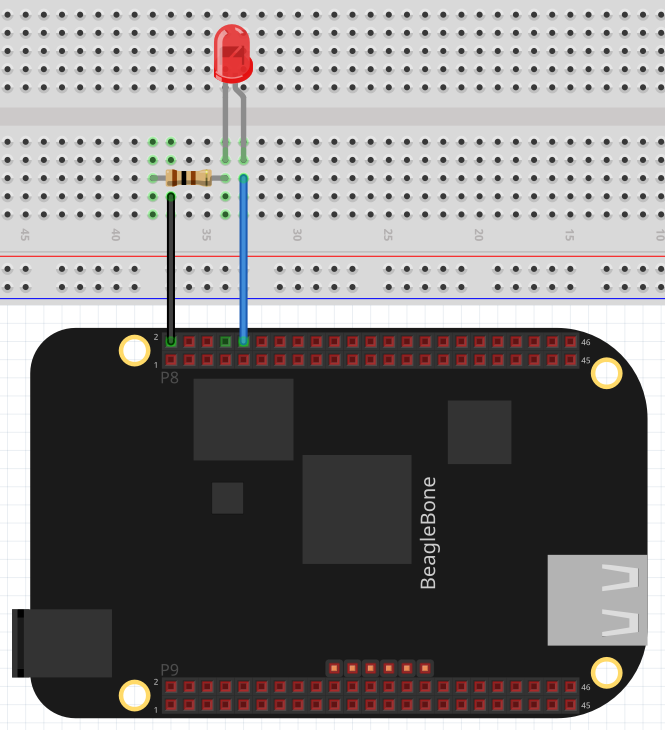
\includegraphics[scale=0.5]{01_beagle_sos.png}
			\caption*{Schemat podłączenia diody do BeagleBone'a}
		\end{center}
	\end{figure}
	\begin{figure}[h!]
		\begin{lstlisting}[language=python]
			import Adafruit_BBIO.GPIO as GPIO
			import time
			
			GPIO.setup("PS_10", GPIO.OUT)
			
			while(True):
			for i in range(12):
			if i % 2 == 0: GPIO.output("P8_10", GPIO.HIGH)
			else: GPIO.output("P8_10", GPIO.LOW)
			if i > 4: t = 1
			else: t = 0.2
			time.sleep(t)
		\end{lstlisting}
		\caption*{Kod użyty do zadania "S.0.S"}
	\end{figure}
	
	\newpage
	
	\section*{Źródła}
	\begin{enumerate}
		\item \href{https://forum.fritzing.org/}{Fritzing}
		\item Materiały podane przez prowadzącego na platformie ekursy.
		\item \href{https://github.com/adafruit/Fritzing-Library/blob/master/parts/BeagleBone%20Black.fzpz}{BeagleBone Black.fzpz} 
	\end{enumerate}
	\begingroup
	\hypersetup{hidelinks}
	\tableofcontents
	\endgroup
\end{document}
